\documentclass[punct]{beamer}
\usefonttheme{professionalfonts}   % 数学公式字体

\titlegraphic{
\includegraphics[width=2cm]{tjnu.jpg}}

\usepackage{color}
%\lineskip=9pt
\linespread{1.3}\selectfont
\makeatletter
\renewcommand\normalsize{%
	\@setfontsize\normalsize\@xpt\@xiipt
	\abovedisplayskip 3\p@ \@plus3\p@ \@minus3\p@
	\abovedisplayshortskip \z@ \@plus3\p@
	\belowdisplayshortskip 3\p@ \@plus3\p@ \@minus1\p@
	\belowdisplayskip \abovedisplayskip
	\let\@listi\@listI}
\makeatother
\parskip=6pt
\usepackage{ctex}
%\usepackage[UTF8, heading = false, scheme = plain]{ctex}
%%%=== theme ===%%%
\usetheme{Madrid}
\useinnertheme{circles}
\setbeamertemplate{navigation symbols}{}
%\setbeamertemplate{footline}[page number]
\setbeamertemplate{footline}[frame number]{}
\usepackage{lmodern}
\usepackage{amsmath}
\usepackage{amssymb}
\usepackage{latexsym}
\usepackage{amsthm}
\usepackage{mathrsfs}
\usepackage{tikz}
\usepackage{graphicx}



\setbeamertemplate{theorems}[]
\newtheorem{thm}{定理}
\newtheorem{prop}[thm]{命题}
\newtheorem{cor}[thm]{推论}
\newtheorem{defi}[thm]{定义}
\newtheorem{lem}[thm]{引理}

\newtheorem{quest}[thm]{问题}
\newtheorem{conj}[thm]{猜想}
\newtheorem{ex}{例}[section]
\newtheorem{pr}{性质}

\newcommand{\blue}{\textcolor{blue}}
\def\pf{\noindent {\bf 证明\ }}
\def\sol{\noindent {\bf 解\ }}


\def\multiset#1#2{\ensuremath{\left(\kern-.3em\left(\genfrac{}{}{0pt}{}{#1}{#2}\right)\kern-.3em\right)}}



\begin{document}

	\title{组\ 合\ 数\ 学\ \  --- \  \  Catalan数}

	\author{张\ 彪}
	\institute[数学科学学院]{\normalsize 天津师范大学}
	%\date[2011年10月13日]{\small 2011年10月13日}
	\date[]{zhang@tjnu.edu.cn}
	\frame[plain]{\titlepage}
%	\begin{frame}{Catalan数}
%		\tableofcontents
%	\end{frame}
%	\AtBeginSection[]
%	{
%		\begin{frame}
%			\frametitle{Outline}
%			\tableofcontents[currentsection]
%		\end{frame}
%	}
%

\begin{frame}
\begin{block}{引例 (姐妹洗碗问题)}

姐姐和妹妹一起洗 4 个碗, 姐姐洗好的碗一个一个往上摆, 妹妹再从最上面一个一个地拿 走放入碗柜摆成一摞, 姐姐一边洗, 妹妹一边拿, 那么妹妹摞好的碗一共有多少种不同的方法?
\end{block}

\begin{minipage}{0.45\linewidth}
\begin{figure}[h]
	\centering
	
\includegraphics[width=0.5\linewidth]{xiwan-1.png}
	\caption{姐妹洗碗问题}
\end{figure}
\end{minipage}
\pause
\begin{minipage}{0.5\linewidth}
 例如
  \begin{itemize}
 \item  姐姐洗2个碗,
 \item 妹妹 摞1个碗,
\item  姐姐 再  洗2个碗,
\item 妹妹 再 摞3个碗.
  \end{itemize}


怎么去描述数学的语言这种取法?

\end{minipage}

\pause
\begin{itemize}
    \item 令$j$为姐姐洗完的碗的个数,$i$为 妹妹摞碗的个数

    \item     条件为妹妹摞碗的个数不能超过姐姐洗完的碗的个数,即$i\le j$

    %    \item 要求摞法的方案数实际上是求从坐标(0,0)到坐标(5,5)的所有满足条件的路径数.
\end{itemize}
上面例子可以叙述为如下的过程
\begin{center}
 $(0, 0) \rightarrow (0, 2)
\rightarrow (1, 2)
\rightarrow (1, 4)
\rightarrow (4, 4)$
\end{center}


\end{frame}


\begin{frame}
    \begin{block}{引例 (姐妹洗碗问题)}

        姐姐和妹妹一起洗 4 个互不相同的碗, 姐姐洗好的碗一个一个往上摆, 妹妹再从最上面一个一个地拿 走放入碗柜摆成一摞, 姐姐一边洗, 妹妹一边拿, 那么妹妹摞好的碗一共有多少种不同的方法?
    \end{block}
     令$j$为姐姐洗完的碗的个数, $i$为 妹妹摞碗的个数, 条件转化为$i\le j$



\begin{minipage}{0.55\linewidth}



    \begin{itemize}
        \item 纵坐标表示姐姐洗完的碗的个数,横坐标表示妹妹摞碗的个数,
            \item 要求摞法的方案数实际上是求从坐标(0,0)到坐标(4,4)的所有满足条件的路径数.
    \end{itemize}

\end{minipage}
 \begin{minipage}{0.4\linewidth}
        \begin{figure}[h]
            \centering
            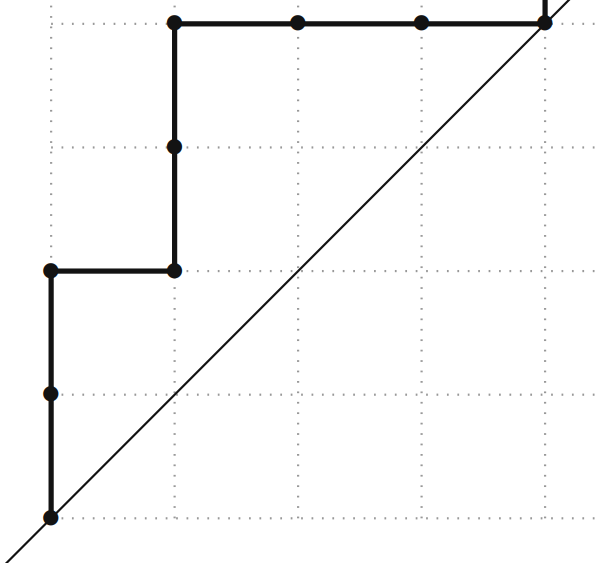
\includegraphics[width=0.6\linewidth]{path.png}
        \end{figure}
 \end{minipage}



\end{frame}


\section{Dyck路的计数}
%\begin{frame}{Dyck 路}
%	\begin{defi}[Dyck 路]
%		从$(0,0)$到$(2n,0)$的格路, 只允许$\nearrow$和$\searrow$的步出现, 且只能走在$x$轴上方, 可简记为 $n$-Dyck 路.
%	\end{defi}
%\begin{figure}[h]
%	\centering
%	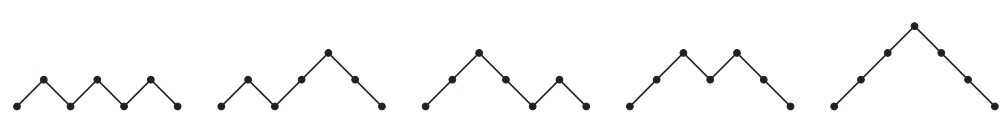
\includegraphics[width=0.8 \linewidth     ]{Dyck-path.jpg}
%	\caption{ Dyck 路(n=3)}
%\end{figure}
%\end{frame}


\begin{frame}
\begin{defi}[Dyck 路]
        一个长度为$2n$的Dyck路是一个从$(0,0)$到$(n,n)$的格路,它
        \begin{itemize}
            \item 含有$n$个水平步骤``E'' \ $(i, j) \rightarrow (i + 1, j)$

            \quad 和$n$个垂直步骤``N'' \ $(i, j) \rightarrow (i, j + 1)$,
            \item 且路径上所有整数格点满足$i\le j$,
            即在平面中位于$y = x$以上.
        \end{itemize}
\end{defi}


\begin{minipage}{0.55\linewidth}
\begin{figure}[h]
    \centering
    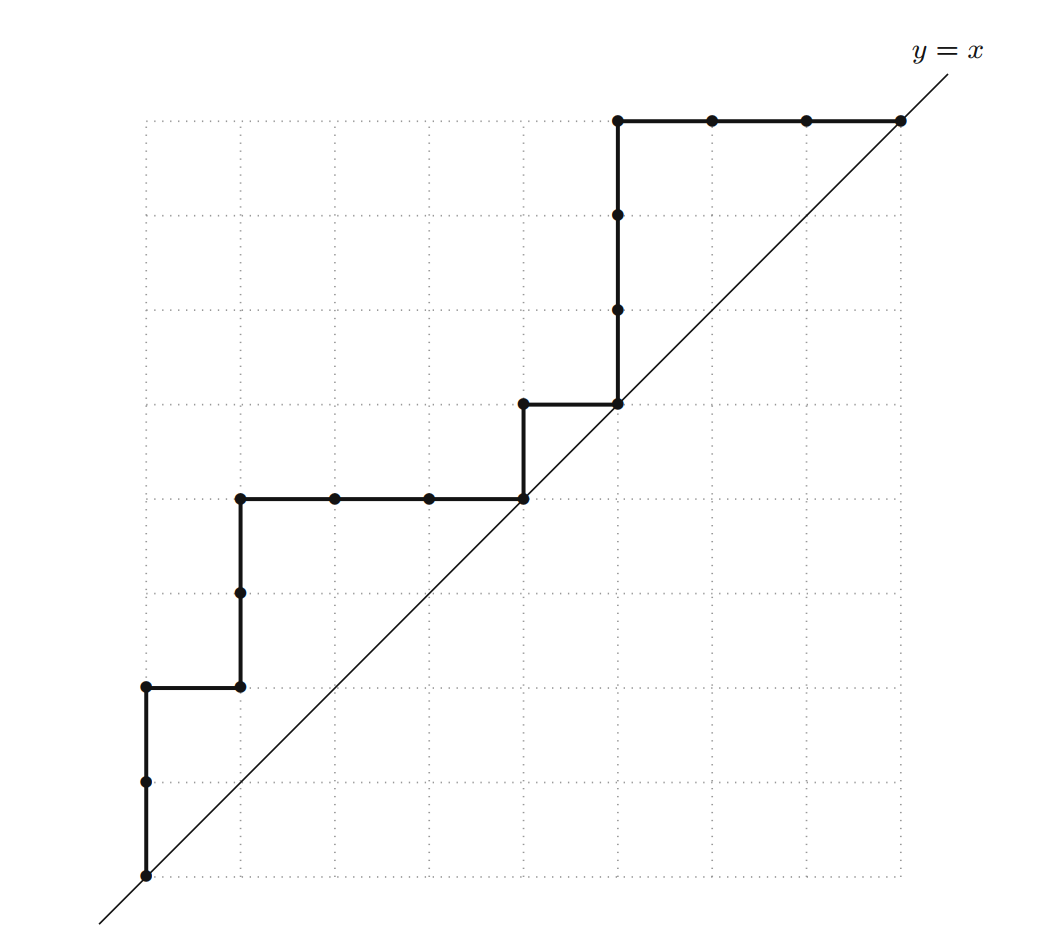
\includegraphics[width=0.8\linewidth]{path-8.png}
    \caption{Dyck 路($n=8$)}
\end{figure}
\end{minipage}
\begin{minipage}{0.4\linewidth}
\pause
我们可以画出
\begin{itemize}
\item 格路的\alert{图}
或
\item 遵循路径的步骤列表写成一个多重集合$\{N, E\}$的\alert{排列}.
\end{itemize}




例如,左边的Dyck路所对应的多重集合$\{N, E\}$的\alert{排列}如下
$$NNENNEEENENNNEEE$$如图所示.
\end{minipage}





\end{frame}



\begin{frame}
%    {Dyck 路}
%\begin{defi}[Dyck 路]
%	从$(0,0)$到$(n,n)$的格路, 只允许$\uparrow$和$\rightarrow$的步出现, 且不能在直线$y=x$的下方.
%
%    \pause
%\end{defi}
\begin{figure}[h]
	\centering
	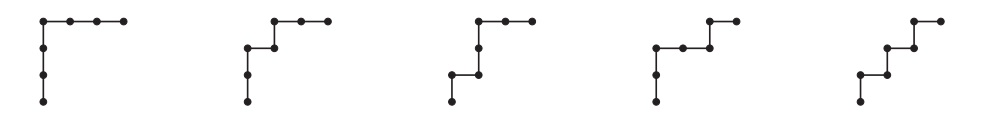
\includegraphics[width=0.9\linewidth]{n-Dyck-path.jpg}
	\caption{Dyck 路($n=3$)}
\end{figure}

我们用$\mathcal{D}(n)$表示长度为$2n$的 Dyck 路的集合, 且定义\textsl{Catalan数}如下
$$
C_n =\# \mathcal{D}(n).
$$
我们将证明,
\begin{thm}
第 $n$ 项 Catalan 数的表达式为
$$C_{n}=\frac{1}{n+1}{2n\choose n}=\frac{2 n !}{n !(n+1) !}=\prod_{k=2}^n \frac{n+k}{k}.$$
\end{thm}



%以我国蒙古族数学家明安图 (1692-1763)和比利时的数学家欧仁·查理·卡塔兰 (1814–1894)的名字来命名.

历史上,清代数学家明安图(1692-1763)在其《割圆密率捷法》最早用到“卡塔兰数”,远远早于比利时的数学家卡塔兰(1814–1894).

有中国学者建议将此数命名为“明安图数”或“明安图--卡塔兰数”.


\end{frame}


\begin{frame}
    经过计数, 可得
    $C_{1}=1, C_{2}=2, C_{3}=5,
    C_{4}=14$.

    \begin{figure}[h]
        \centering
        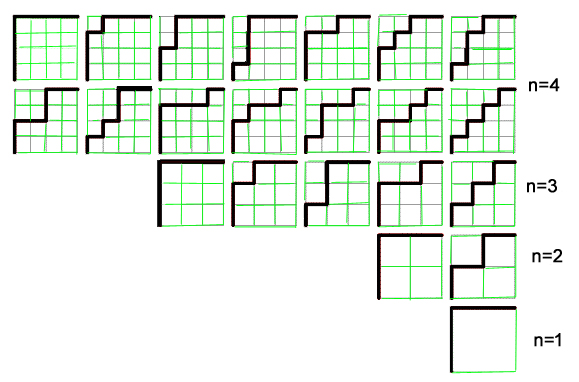
\includegraphics[width=0.95\linewidth]{Dyck-4.jpeg}
        %    \caption{Dyck 路}
    \end{figure}
\end{frame}

\section{生成函数求解Catalan数表达式}
\begin{frame}{递推关系的建立}
    以半$n$长Dyck 路为例. 设满足条件的Dyck 路的条数即Catalan数为$C_{n}$. 设满足条件的一条Dyck 路: $P=v_{0}v_{1}\cdots v_{2n},$
    其中$v_{0}=(0,0)$,$\ v_{2n}=(n,n)$.

\begin{minipage}{0.4\linewidth}
    \begin{figure}[h]
        \centering
        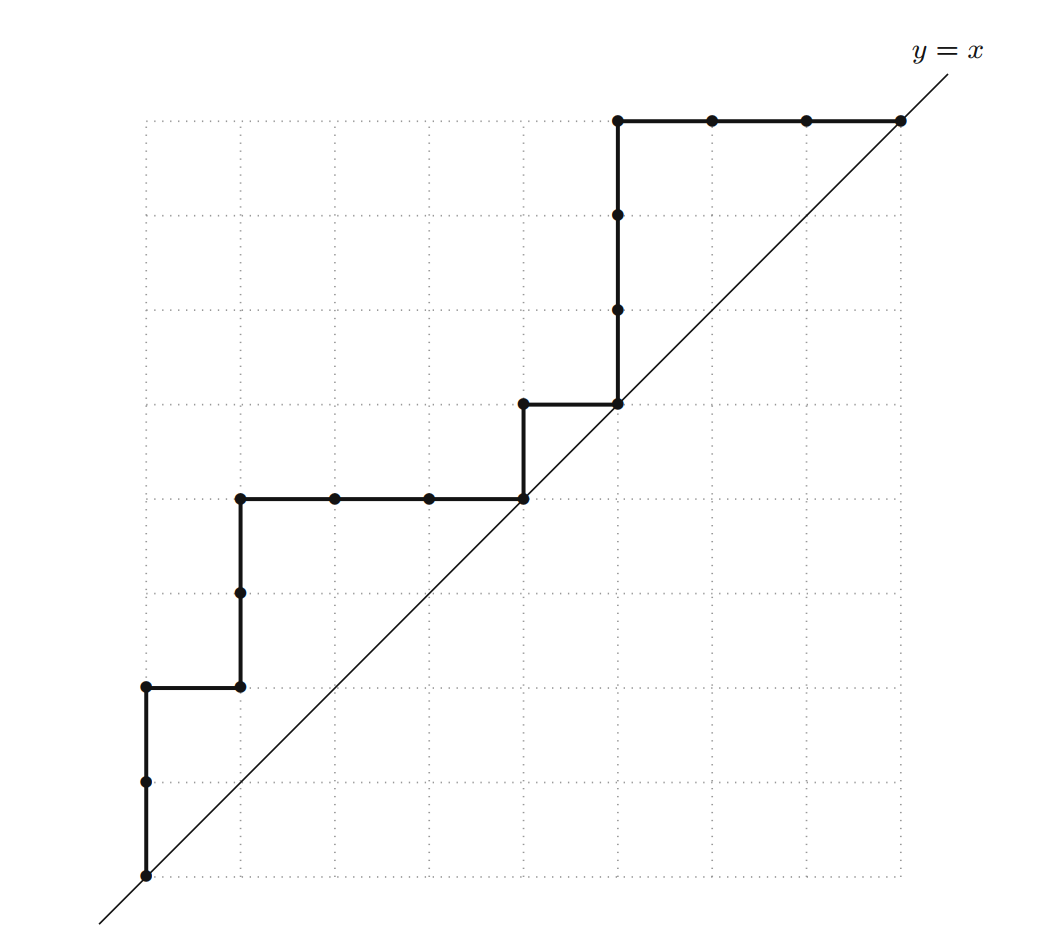
\includegraphics[width=0.8\linewidth]{path-8.png}
        \caption{Dyck 路($n=8, i=4$)}
    \end{figure}
\end{minipage}
\begin{minipage}{0.55\linewidth}
    设\alert{第一个}与$y=x$相交的顶点为$v_{2i}=(i,i)$. 将Dyck 路 $P$按照$v_{2i}$分成两段,
    \begin{enumerate}
        \item $v_{0}=(0,0)\rightarrow v_{2i}=(i,i)$. 此时第一步一定向上, 最后一步一定向右, 故只需考虑$(0,1)\rightarrow (i-1,i)$的格路条数, 计数为$C_{i-1}$.
        \item $v_{2i}=(i,i)\rightarrow v_{2n}=(n,n)$. 计数为$C_{n-i}.$
   \end{enumerate}
\end{minipage}

    于是有
    \\[-20pt]
    \[
    C_{n}=\sum_{i=1}^n C_{i-1}C_{n-i}.\tag{1}
    \]
\end{frame}


\begin{frame}
    设$C_{n}$为Catalan数, 规定 $C_{0}=1$.
    令\[
    A(x)=\sum_{n=0}^{\infty}C_{n}x^{n}.
    \]对(1)式两边同乘以$x^{n}$并关于$n\geq0$求和得
    \[
    A(x)-1=xA(x)^{2},
    \]解得\[
    A(x)=\frac{1\pm \sqrt{1-4x}}{2x}.
    \]

%    若取``+", 则当$x\rightarrow0$时, $A(x)$不存在, 故舍去.
%
%    但若取``$-$",则可利用洛必达法则, 当$x\rightarrow0$时, $A(x)\rightarrow 1$.
     利用二项式定理
    $$
    \sqrt{1-4 x}=(1-4 x)^{\frac{1}{2}}=\sum_{n \geq 0}\binom{\frac{1}{2}}{n} \left(-4x\right)^n .
    $$

\end{frame}

\begin{frame}
       因此,
    \begin{align*}
   A(x) & =\frac{1-\sqrt{1-4x}}{2x}        \quad \mbox{(舍去正号,为什么?)} \\[5pt]
        &=\frac{1}{2 x}\left(1-\sum_{n \geq 0}\binom{\frac{1}{2}}{n}(-4 x)^n\right) \\[5pt]
        &=-\frac{1}{2} \sum_{n \geq 0}\binom{\frac{1}{2}}{n+1}(-4)^{n+1} x^n \\[5pt]
        &= \sum_{n\ge 0}\frac{1}{n+1}\binom{2n}{n} x^n.      \quad \mbox{(计算过程请自行补充完整)}
    \end{align*}
    提取 $x^n$ 项系数, 得
\begin{align*}
 C_n
& =\frac{1}{n+1}\binom{2n}{n} .
\end{align*}


\end{frame}



\section{Catalan数的组合解释}


\begin{frame}{建立$n+1$个$x$组成的括号字符串}
    一个$n+1$个$x$组成的括号字符串由插入$n$个左括号和$n$个右括号组成.
    %, 满足字符串上的$n$位二进制.

    $n=3$时,
    \[
    x(x(xx)) \quad x((xx)x)\quad (xx)(xx)\quad (x(xx))x\quad ((xx)x)x
    \]
    \begin{block}{注}
        对于(((xx)x)((xx)(xx)))这种形式的元素, 我们通常忽略最左和最右的括号.
    \end{block}
    % \begin{figure}[h]
        % 	\centering
        % 	\includegraphics[width=0.6\linewidth]{.jpg}
        % 	%\caption{}
        % \end{figure}
\end{frame}



\begin{frame}{$2n$长Ballot序列}
    设$w=w_{1}\cdots w_{2n}$是由$n$个1和$n$个2组成的序列, 对任意$i=1,2,\cdots, 2n$,  要求前$i$个字$w_{1}\cdots w_{i}$ 中1的个数大于或等于2的个数. 满足上述条件的序列称为 $2n$ 长 Ballot 序列.

    如$n=3$时, Ballot序列如下
    \[
    111222\quad 112122\quad 112212\quad 121212\quad 121122
    \]
\end{frame}
\begin{frame}{$n$ 对圆括号合法排列}
    $n$ 对圆括号排在一起, 从左往右看, 左括号的个数大于等于右括号的个数, 则称为合法.

    $n=3$时,
    \[
    ((()))\quad (()())\quad (())()\quad ()()()\quad ()(())
    \]
    \begin{block}{注}
        Catalan数任意两个组合解释之间都可建立双射. 这里Ballot序列与$n$对圆括号合法排列之间的双射, 只需将 ``1" 与 ``(" , ``2" 与 ``)" 对应起来即可.
    \end{block}
\end{frame}




\begin{frame}{凸$n+2$边形切割}
	\begin{itemize}
		\item 将$n+2$边形添加对角线, 使其被切割为$n$个三角形.
	\end{itemize}
	\begin{figure}[h]
		\centering
		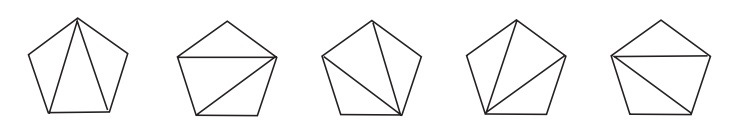
\includegraphics[width=0.8\linewidth]{Triangulated-polygons.jpg}
		\caption{凸$n+2$边形切割($n=3$)}
	\end{figure}
\end{frame}

\begin{frame}{$n$个顶点的二叉树}
	\begin{itemize}
		\item 树:连通且无圈.
		\item 二叉树:顶点度小于等于2的树.
	\end{itemize}
	\begin{figure}[h]
		\centering
		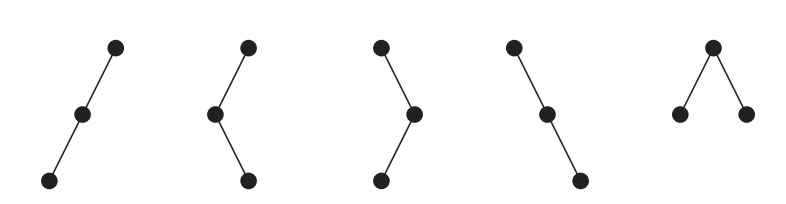
\includegraphics[width=0.8\linewidth]{binary-trees.jpg}
		\caption{$n$个顶点的二叉树($n=3$)}
	\end{figure}
\end{frame}



\begin{frame}{$n+1$个$x$组成的括号字符串与$n$-二叉树间的双射}
    \begin{itemize}
        \item 设$n+1$个$x$组成的括号字符串为$w$, 定义二叉树$B_w$的递推关系满足:如果$n=0$,则$B_w=\emptyset$;
        否则, 从$w$最外层括号开始, 如果$w=st$, 则$B_w$有一个根顶点$v$、左子树$B_s$及右子树$B_t$.
        例如, 如果$w=xx$, 则$B_w$只包含一个顶点(根). 对下图中的二叉树, 其对应的括号为
        \[
        ((xx)x)x \quad (x(xx))x \quad x((xx)x)\quad x(x(xx)) \quad (xx)(xx)
        \]
    \end{itemize}
    \begin{figure}[h]
        \centering
        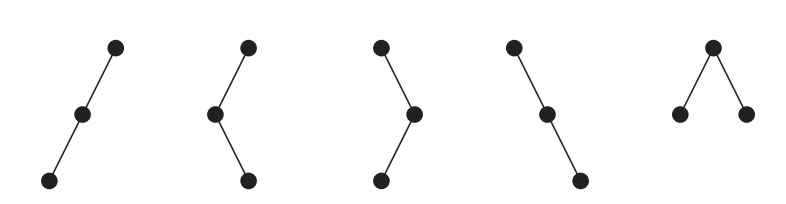
\includegraphics[width=0.6\linewidth]{binary-trees.jpg}
        \caption{$n$个顶点的二叉树(n=3)}
    \end{figure}
\end{frame}



\begin{frame}{建立$n$-二叉树与凸$n+2$边形切割间双射}
	\begin{itemize}
		\item 固定多边形的边$e$, 在$T$的每个三角形内部放置一个顶点, 让根顶点对应于以$e$为边的三角形.
		连接相邻三角形中的点, 如图$(a)$. 从顶点$v$出发, 确定边$f_1$及$f_2$, 沿着边$f_1$逆时针旋转定义第一条边为左侧边$f_{11}$,第二条边为右侧边$f_{12}$.
		以此类推, 即可得到二叉树如$(b)$.
	\end{itemize}
	\begin{figure}[h]
		\centering
		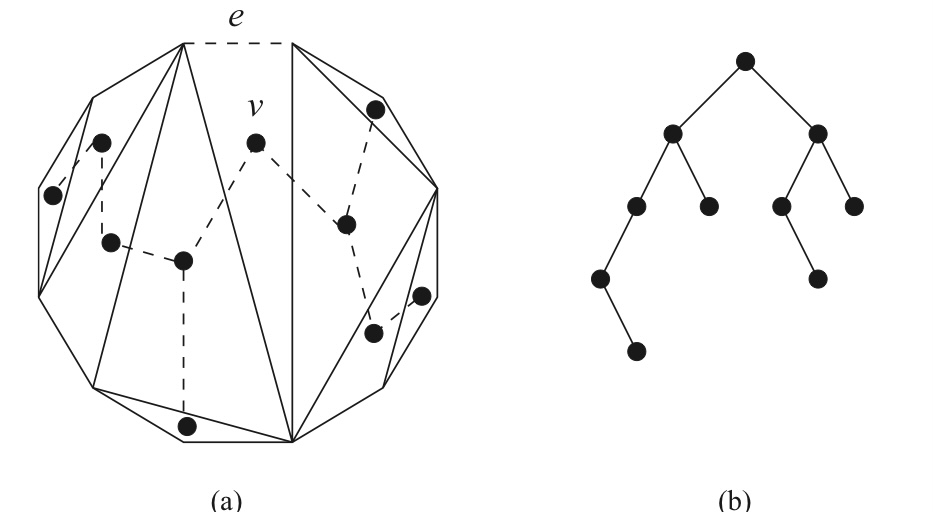
\includegraphics[width=0.6\linewidth]{triangulationsT-b.jpg}
		%\caption{}
	\end{figure}
\end{frame}

% \begin{frame}{$a_i \leq i $的整数序列}
% 	整数序列满足$1\leq a_1 \leq \cdots \leq a_n$, 其中$a_i \leq i$.

% 	$n=3$时, 序列$\{a_n\}$如下
% 	\[
% 	111\quad 112\quad 113\quad 122\quad 123
% 	\]
% \end{frame}






%
%
%\section{组合方法求解Catalan数表达式}
%\begin{frame}{一种组合方法}
%    \begin{thm}第 $n$ 项 Catalan 数
%        $$C_n={2n\choose n}-{2n\choose n-1}.$$
%    \end{thm}
%    {\bf{证明}} 定理中这个等式可以借助 Dyck 路
%    通过组合方法来证明. 这里, 我们给出的是一种应用了反射原理的证明方法.
%\end{frame}
%\begin{frame}{一种组合方法}
%    \begin{itemize}
%        \item 	令 $A$ 是平面上从 (0, 0) 到 $(2n, 0)$ 且每步只能取 (1, 1) 或 $(1,
%        -1)$ 的路的集合. 易知 $|A|={2n\choose n}$. 令 $B$ 是 $n$-Dyck 路
%        的集合, 则 $|B|=C_n$ (第 $n$ 项 Catalan 数). 令 $C$ 是包含于 $A$
%        且穿越了 $x$ 轴的那些路的集合, 则 $|C|=|A|-|B|$. 令 $D$ 是平面上从
%        (0, 0) 到 $(2n, -2)$ 且每步只能取 (1, 1) 或 $(1, -1)$
%        的路的集合. 易知 $|D|={2n\choose n-1}$.
%        \item 因此我们只需要说明 $|C|=|D|$
%        即可. 对 $C$ 中任意一条路 $p$, 假定 $(2i-1, -1)$ 是 $p$ 与 $y=-1$
%        所交的第一个点, 容易知道, 将 $p$ 中从 $(2i-1, -1)$ 到 $(2n, 0)$
%        的那段关于 $y=-1$ 作反射, $(0, 0)$ 到 $(2i-1,
%        -1)$那段不变所得到的是从 $(0, 0)$ 到 $(2n, -2)$ 属于 $D$ 的路
%        $p'$, 很容易证明这样的反射事实上给出了集合 $C$ 和 $D$
%        间的一个一一对应. \qed
%    \end{itemize}
%
%\end{frame}
%
%


\end{document}